\documentclass[10pt, handout, xcolor=table]{beamer}

\usepackage[utf8]{inputenc}
\usepackage{amsmath}
\usepackage{amsfonts}
\usepackage{amssymb}
\newcommand*\themecol{\usebeamercolor[fg]{structure}}

\setbeamertemplate{navigation symbols}{}
 \setbeamertemplate{footline}[frame number]



\usepackage{tikz}
\usetikzlibrary{shapes.geometric, arrows}
\tikzstyle{prob} = [rectangle, minimum width=3cm, text width = 4.5cm, minimum height=1cm, text centered, draw=black, fill= blue!20]
\tikzstyle{stat} = [rectangle, minimum width=3cm,  text width = 4.5cm, minimum height=1cm, text centered, draw=black, fill= red!20]
\tikzstyle{arrow} = [thick,->,>=stealth]


\setlength{\parindent}{0pt}
\setlength{\parskip}{6pt}

\title{STAT 111\\
{\small Recitation 2}}

\author{Mo Huang}
\institute{Email: mohuang@wharton.upenn.edu \\
\vspace{0.25cm}
Office Hours: Wednesdays 3:00 - 4:00 pm, JMHH F96\\
\vspace{0.25cm}
Slides (adapted from Gemma Moran): \url{github.com/mohuangx/STAT111-Fall2018} }


\date{September 14, 2018}


\begin{document}

\begin{frame}
\titlepage
\end{frame}


\begin{frame}{Parameters ($\theta$), Random Variables ($X$), and Data ($x$)}
\begin{itemize}\itemsep1ex
\item<1-> A {\themecol parameter} represents some underlying numerical constant of a phenomenon. Represented by Greek letters.
\item<3-> A {\themecol random variable} is a numerical outcome of interest in a future experiment. Can be modeled by a probability {\themecol distribution} which depends on the parameter. Represented by capital letters.
\item<5-> {\themecol Data} is the realization or observed value of a random variable after performing the experiment. Represented by lower-case letters.
\end{itemize}

\bigskip
\only<2->{Fair coin-flipping example:}
\begin{itemize}\itemsep1ex
\item<2-> A {\themecol parameter} $\theta$ is the underlying probability of obtaining a head. $\theta = 0.5$.
\item<4-> A {\themecol random variable} $X$ is the number of heads obtained in 10 tosses. Can be modeled by a binomial distribution dependent on $\theta$.
\item<6-> {\themecol Data} $x=6$ is observing 6 heads in 10 tosses, a realization of $X$.
\end{itemize}
\end{frame}

\begin{frame}{Random Variables}
\begin{itemize}\itemsep1ex
\item<1-> Two types of random variables: {\themecol discrete} and continuous.
\item<1-> A {\themecol discrete random variable} is a random variable that can only take on a countable set of numbers.
\item<1-> The {\themecol probability distribution} of a discrete random variable is the range of values it can take \emph{and} the probabilities of these values.
\item<2-> For example:
\begin{itemize}
\vspace{0.25cm} \color{blue!70}
\item Let $X$ be the number of heads I toss if I toss a fair coin 3 times.
\end{itemize}
\end{itemize}
\uncover<3->{
\begin{table}
\begin{tabular}{|c|c|c|c|c|}
\hline
\rowcolor{blue!10} $x$ & 0 & 1& 2&3  \\ \hline
$P(X = x)$ & 0.125 & 0.375 & 0.375 &0.125 \\
\hline
\end{tabular}
\caption{Probability distribution of $X$ using the tableau method.} 
\end{table}}
\end{frame}



\begin{frame}{The Binomial Distribution}
\begin{itemize}
\setlength{\itemsep}{15pt}
\item The {\themecol binomial distribution} arises if:
\begin{enumerate}
\vspace{0.25cm}
\setlength{\itemsep}{6pt}
\item<2-> We plan to conduct a fixed number of experiments. We denote the number of experiments as $n$.
\item<3-6,8-> In each experiment, there are two outcomes: ``success'' or ``failure".
\item<4-6, 9-> The experiments are independent.
\item<5-6, 10-> The probability of a success is the same for each experiment.
\end{enumerate}
\item<6-> For example: 
\begin{enumerate} \color{blue!70}
\vspace{0.25cm}
\setlength{\itemsep}{6pt}
\item<7-> I plan to toss a coin $n$ times.
\item<8-> I can toss either a head or a tail.
\item<9-> Each coin toss is independent of the next - it doesn't matter whether I get a head or a tail on the previous toss.
\item<10-> The probability of getting a head is the same for each toss.
\end{enumerate}
\end{itemize}
\end{frame}

\begin{frame}{The Binomial Distribution}
\begin{itemize}
\setlength{\itemsep}{15pt}
\item Let $X$ be a binomial random variable where $\theta = P(\text{success})$ and there are $n$ experiments. Then the probability distribution of $X$ is given by:
$$ P(X = x) = {n \choose x} \theta^x (1-\theta)^{n-x}, \quad \text{for } x = 0, 1, 2, \dots, n.$$
\begin{itemize}
\setlength{\itemsep}{6pt}
\item<2-> $\theta$ is called a {\themecol parameter}: a constant whose value may be known or unknown.
\item<3-> ${n \choose x} = \frac{n!}{x!(n-x)!}$ is said as ``$n$ choose $x$'': it is the number of ways $x$ successes can occur in $n$ experiments.
\end{itemize}
\item<4->[Note:] $X \sim \mathcal{B}(n, \theta)$ means ``$X$ is a binomial random variable with $n$ experiments and probability of success $\theta$.''
\end{itemize}
\end{frame}

\begin{frame}{The Binomial Distribution: Questions}
\begin{itemize}
\setlength{\itemsep}{15pt}
\item[Q1:] Let $X$ be the number of heads if I toss an unbiased coin 3 times ($n = 3, \theta = 0.5$). Find the probability distribution of $X$ in ``tableau" form.
\item<2->[A1:] \color{red}  
\end{itemize} 
\uncover<2->{ \color{red} {
\begin{columns}
\begin{column}{0.5\textwidth}
\begin{align*}
P(X = 0) &= {3 \choose 0} (0.5)^0 (0.5)^3 \\
&= 0.125 \\
P(X = 1) &= {3 \choose 1} (0.5)^1(0.5)^2 \\
&= 0.375 
\end{align*}
\end{column}
\begin{column}{0.5\textwidth}
\begin{align*}
P(X = 2) &= {3 \choose 2} (0.5)^2(0.5)^1 \\
&= 0.375 \\
P(X = 3) &= {3 \choose 3} (0.5)^3 (0.5)^0 \\
&= 0.125
\end{align*}
\end{column}
\end{columns}}
}

\uncover<3->{ \color{black}
\begin{table}
\begin{tabular}{|c|c|c|c|c|}
\hline
\rowcolor{blue!10} $x$ & 0 & 1& 2&3  \\ \hline
$P(X = x)$ & 0.125 & 0.375 & 0.375 &0.125 \\
\hline
\end{tabular}
\caption{Probability distribution of $X$ using the tableau method.} 
\end{table}}
\end{frame}

\begin{frame}{The Binomial Distribution: Tables}
\begin{itemize}
\setlength{\itemsep}{6pt}
\item[Q2:] $X\sim \mathcal{B}(18, 0.15)$. Find $P(X = 4)$.
\item<2->[A2:] {\color{red} $P(X = 4) = 0.1592$}
\begin{figure}
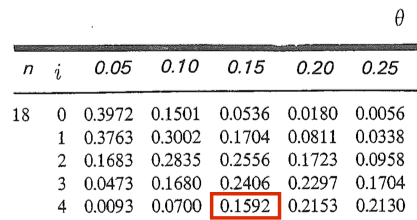
\includegraphics[width = 0.5\textwidth]{images/rec2_1}
\end{figure}
\item<3->[Q3:] Find $P(X \leq 4)$.
\item<4->[A3:] {\color{red} 
\begin{align*}
P(X \leq 4) &= P(X= 0) + P(X=1)+P(X=2)+P(X=3)+P(X=4) \\
&= 0.0536 + 0.1704 + 0.2556 + 0.2406 + 0.1592 \\
&= 0.8794
\end{align*}}
\end{itemize}
\end{frame}

\begin{frame}{The Binomial Distribution: Tables}
\begin{itemize}
\setlength{\itemsep}{6pt}
\item<1->[Q2:] $X\sim \mathcal{B}(12, 0.8)$. Find $P(X = 3)$.
\item<2->[A2:] \color{red} Finding 3 successes with $\theta = 0.8$ is the same as finding 9 failures with $\theta$ of failure $0.2$. Hence, $P(X = 3) = 0.0001$.
\begin{figure}
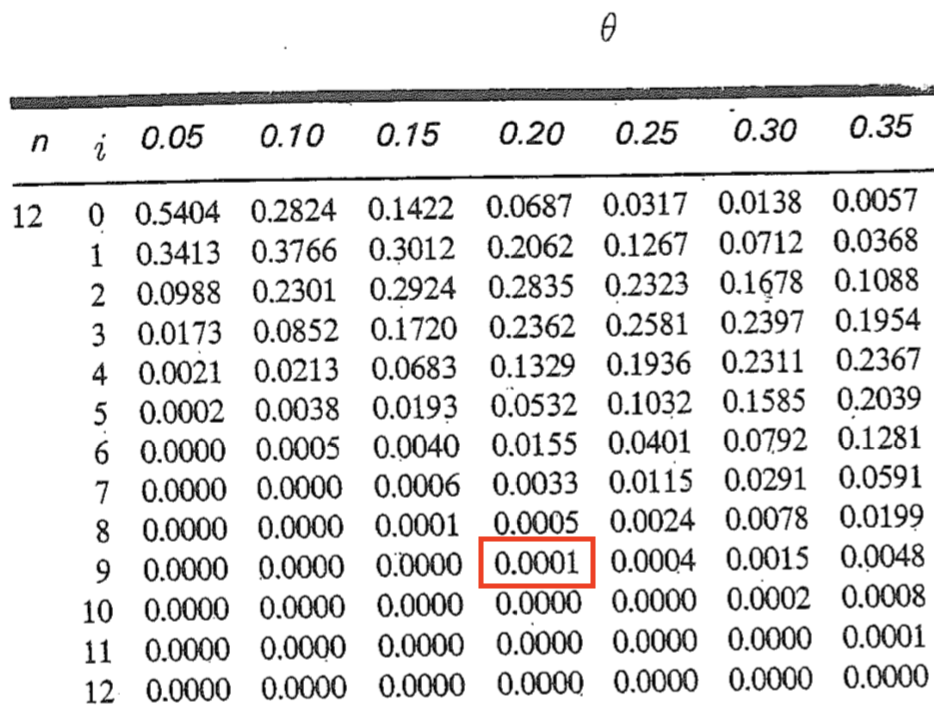
\includegraphics[width = 0.7\textwidth]{images/rec2_2}
\end{figure}
\end{itemize}
\end{frame}


\begin{frame}{Random Variables: Mean}
\begin{itemize}
\setlength{\itemsep}{15pt}
\item<1-> The {\themecol mean of a random variable} (expected value) is the long-run average of realizations of the random variable over repeated experiments.
\item<2-> This mean of random variable $X$ is different from the sample mean, which is the average of a \emph{finite} number of observations ($x$).
\item<3-> Let $X$ be a discrete random variable that can take values $\{v_1,v_2,\dots, v_k\}$. Then the mean of $X$ is given by:
\begin{align*} 
\mu &= \sum_{i = 1}^k v_i P(X = v_i)\\
&= v_1P(X = v_1) + v_2P(X = v_2) + \cdots + v_kP(X = v_k).
\end{align*}
\begin{itemize}
\item[Note:] We use $\mu$ to denote the mean of a random variable.
\item[Note:] Can think of it as a weighted average, weighted by probability.
\end{itemize}
\end{itemize}
\end{frame}

\begin{frame}{Random Variables: Questions}
\begin{itemize}
\setlength{\itemsep}{6pt}
\item[Q2:] Let $X$ be the outcome of one roll of a biased dice where the probability of the number $j$ turning up is $j/21$. Find the mean of $X$.
\item<2->[A2:] {\color{red} \begin{align*}
\mu &= 1 \times 1/21 + 2 \times 2/21 + 3 \times 3/21 + 4 \times 4/21 + 5 \times 5/21 + 6\times 6/21 \\
&= 91/21
\end{align*}}
\vspace{-0.5cm}
\item<3->[Q3:] Let $X$ be a binomial random variable with $n = 2$ and $\theta = 0.8$. Find the mean of $X$ using the binomial table.
\vspace{0.5cm}
\item<4->[A3:] {\color{red} 
\begin{align*}
\mu &= 0 \times 0.04 + 1 \times 0.32 + 2\times 0.64 \\
&= 1.6
\end{align*}}
\vspace{-0.5cm}
\end{itemize}
\end{frame}




\begin{frame}{The Binomial Distribution: Mean}
\begin{itemize}
\setlength{\itemsep}{20pt}
\item For the binomial distribution, we have a simpler formula for the mean: if $X\sim \mathcal{B}(n, \theta)$, then the mean of $X$ is
\begin{align*}
\mu = n\theta.
\end{align*}
\item<2-> For example: 
\begin{itemize}
\item \color{blue!70} On the previous slide, we calculated the mean of a binomial random variable with $n = 2$ and $\theta = 0.8$ to be 1.6. This is exactly $n\theta$. 
\end{itemize}
\vspace{0.5cm}
\begin{itemize}
\item<3->[Note:] This formula is \emph{only} for the binomial distribution.
\end{itemize}
\end{itemize}
\end{frame}

\begin{frame}{Random Variables: Variance}

\begin{itemize}
\setlength{\itemsep}{15pt}
\item<1-> The {\themecol variance of a random variable} is a measure of the \emph{spread} of a distribution - that is, how far away values are from the mean.
\item<2-> Let $X$ be a discrete random variable that can take values $\{v_1,v_2,\dots, v_k\}$. Then the variance of $X$ is given by:
\begin{align} 
\sigma^2 &= (v_1 - \mu)^2P(X = v_1) + \cdots + (v_k - \mu)^2P(X = v_k) \\
&\hspace{3cm} \text{\themecol\emph{or} } \notag\\
\sigma^2&= v_1^2P(X=v_1) + \cdots + v_k^2P(X = v_k) - \mu^2
\end{align} 
\item<3-> The {\themecol standard deviation of a random variable} is the square root of the variance and is denoted by $\sigma$.
\item<3-> For a {\themecol binomial }random variable $X\sim \mathcal{B}(n, \theta)$:
$$\sigma^2 = n\theta(1-\theta)$$
\item<4->[Note:] \small The variance is always positive - you can't have a negative spread of a distribution.
\end{itemize}

\end{frame}


\end{document}


